\chapter{State of the Art review}

\section{Previous and related work}\label{related_work}

\lettrine{T}{he problem} of the analysis scalability is not faced for the first time in 
this paper but there is a previous work in what this thesis is rely and is 
supported on. Several tools are actually being used in order to ease the analyst
work. Talking about structure analysis we can split previous works into two main
subsets. By one hand we have the behavioral structure that want to expose the
different phases on an execution in terms of performance and by the other hand
the syntactic structure that provide information about the actual program
structure such as profiling.

\subsection{Behavioral structure}

If we consider the same bunch of code will behave, in general, in the same
manner it can be assumed that there is a powerful correlation between the
behavior and the code. By this way it can be said a behavioral analysis is a
side-channel analysis because indirectly the internal syntactic structure can be
betrayed. This consideration could be true in some cases but not in general. The 
main goal of the different approaches presented in this section is not
to present a syntactic but a behavioral structure. The motivation is that when
analyst deals with syntactic structure, time variations of the same functions is
hidden. This situation can appears for example when calling same function with
different parameters. For the analyst point of view could be more interesting to
have this information unfolded. Take into account that this same property can
end up identifying different parts of the code as the same phase.

Even if the goal of the approaches explained below does not match perfectly with
goal of this thesis, they provide a really useful insights as a related work.

In \cite{casas2007automatic} they propose, similarly to this paper, 
automatically extract the internal structure of an MPI application from a
Paraver tracefile and provide to analyst just representative phases. 
They rely on signal analysis for this propose. 
Their analysis consists on two main phases:
The first is to clean-up the trace by identify the perturbed regions.
Perturbed regions are those parts of the trace that has been perturbed nor by
the application nor by architecture but by external factors such that unknown
system activity or tracing package. Their clean-up phase is centered on remove
noise from tracing package, i.e. flush to disk. By building up a signal based
on flushing events and transform it by Closing morphological filter they end up
with this perturbed phases. The second phase is the identification of the
phases. It is done by means of autocorrelation and periodicity analysis of a
signal. This signal is build up from any metric like instantaneous FLOPs but the
use number of MPI point to point calls being executed. Once the period is
successfully detected the same process is done recursively on one of the
periods. This allows to have a hierarchical structure. Finally the output is
basically information about the different phases like number of iteration and
timing plus some representative cuts of the original trace. It differs on this
thesis approach basically on the fact that they extract the structure by
behavioral analysis instead of actual callstacks analysis. The main drawback is
this method is not concerning about noise from the actual application so same
phase on code can be detected as different phases, also if there is a lot of
perturbation at level of e.g. cache, depending on what metric is being used, no
structure could be detected. 

Similarly with the previous approach, in 
\cite{gonzalez2013application} is proposed to apply clustering techniques in
order to identify the different execution phases. Different parts of the
execution are considered as the same phase depending on the behavior,
so an analysis using some hardware metrics is
performed. The first phase is about reducing the complexity of the clustering by
filtering the less relevant computation burst, i.e. little bursts according
with a given threshold. In order to reduce the dimensionality the proposal is to
use two different dimension sets: The first one is Completed Instructions
against IPC\footnote{Instructions per cycle}. This configuration provides a
performance view. The second is Completed instructions against L1 and L2 cache
misses. This combination reflects the impact of the architecture on the
application structure. 

\subsection{Syntactic structure}

Syntactic structure is centered on providing the actual program code structure so
it needs to use some debug information about symbols and about the position of
the instruction in code is being executed and monitoring, i.e. the callstack.

The main interest on having the syntactic structure of an application is to be
aware about not just what but where. This is important in the process of who to
blame in code and provides insights of the actual application that with just
behavioral structure can not be presented like for example where do we have
loops and how many iterations performs.

Profile tools are used to present behavior information attached to a 
syntactic structure. Although this is a scalable
solution for performance monitoring, they are used to discard temporal order so
structures like loops are just exposed indirectly by the number of calls metric.
Additionally some sort of bottlenecks like late-sender problems are difficult to
detect without time order information. These following approaches presents the
information in a way that are in the midway between profilers and tracers. In
general starts from a huge trace and by means of summarizing and aggregating
data tries to present the minimum and meaningful information to the analyst.

In \cite{noeth2009scalatrace} they are concerning about the scalability of the
tracing part. Even if they are centered on the logging (or tracing) part their
work is really useful for this thesis purposes. They claim reductions of about a
thousand in terms of trace size just by detecting the structure of the
application, e.g. If the same thing is repeated 100 times, just saving it once
and tagging with the number of times it is executed should be enough. They
propose to use RSD (Regular Section Descriptors) to express MPI events nested
inside a loop and a sequence analysis algorithm loosely based on the SIGMA
scheme for memory analysis for detect the repetitive patterns. Their compression
is done in two phases. The first one is an intra-node compression, where the
repetitive patterns arise and the second one is inter-node merge, where all
single-node compressions are merged forming the whole application trace.
They introduce interesting concepts as calling sequence identification used for
unambiguously identify different MPI calls that lie on different code positions, 
and recursion folding signatures for dealing with recursion. Also they claim
that even if their main target is to compress traces, Scalatrace also can be
used for analyze the application structure by doing a little demo showing how it
can detect the most outer loop iterations or timesteps. One of the main
drawbacks of this approach is that the complexity of both intra-node and
inter-node compression can be of $O(n^2)$.

In the same line as the previous work, Compressed Complete Call Graphs (cCCG) are 
presented by \cite{knupfer2005construction}. It is about finding repetitive 
patterns for loosely or lossless compression but instead of at tracing time, 
over an already traced huge trace. 
This compression will allow to analyst to analyze whole huge traces 
interactively, difficult business when dealing with this amounts of information. 
CCG is basically a graph of function calls of a program so the main structure is
defined by the function call hierarchy while additional information are appended
usually as leaf nodes. The construction phase is quite simple. The trace is
traversed in a sequential manner, every time a function enter event is detected,
new node is generated and append to the current active node. The
other way around when exit function event is read, the current active node is
finalized and all information concerning to this node is presented e.g.
duration. Additionally, while constructing, the graph is compressed. The basic 
idea is to replace $n$ repeated sub-trees that are equal or similar with a 
reference to a single instance saving $n-1$ remaining copies. For similar is
understood that when comparing nodes not all properties must be equal for
example is not needed some scalar values like duration match perfectly (some
configured deviation is acceptable) but properties like function id must. They
claim main compression ration about 200 can be achieved with this approach.
Additionally this compression technique does not need to uncompress anything, the
user (or any analysis algorithm) just can traverse the graph and gather
information.

This approach improves profiling in the sense that same function with same call
path and different time behaviour is exposed to analyst but still presents a lack 
of information on the order of the execution of the different graph paths.In
\cite{aguilar2016event} they present the Event Flow Graphs (EFG) as an intent of
provide temporal order between events. In this case they are centered on
syntactic structure but just focused on MPI operations. EFG are
weighted directed graphs where every node is an MPI call and edges the
transitions between them, so the program code blocks executed between them.
Graph nodes can contain aggregate information like call duration or message size
and edges can be attached with information about CPU burst like performance
metrics like IPC additionally to the number of times the edge is traversed.
Now let's imagine we have a loop where there are three MPI calls $A$, $B$ and
$C$ and $B$ and $C$ are mutual exclusively executed so if we have 10 
iterations we have $A*10$, $B*5$ and $C*5$. In order to reconstruct the execution
we need information about in what iterations B and C have been executed.
So additionally they present temporal-EFG that introduce more
information for these cases where the execution order can not be reconstructed
with the previous EFG. They claim this technique can be used for trace
compression, application structure detection and visual performance analysis.
Following with application structure detection, what is where this thesis is
focused on, they use algorithms for cycle detection over the t-EFG (DFS-based)
and once cycles are detected the graph is transformed to a hierarchical tree
where loops and subloops are showed up. Statistics about loops can be gathered
like number of iterations, total time in loops and so on.

Even if they use code position information for building up they EFG (as it can
be seen in previous publication \cite{aguilar2014mpi}) they are not pushing it
to analyst so it is not clear how they are relating EFG with source code for the
analysis.

In \cite{trahay2015selecting} they present an approach for select points of
interest automatically, understanding as points of interest these iterations that
behave different from the majority. The first phase is a post-mortem analysis of
a given trace. This analysis is about finding patterns of events that are
repeated, i.e. folding loops that has been unfolded during the
tracing\footnote{Unfolding in the sense that tracing process represent loops as
a sequence of a repeated set of events.}. Their algorithm is about finding short
repeated sequences of events and try to expand the pattern. After detect the
intern structure of an application, the distribution of durations of the
different iterations of the detected loops is an arbitrary construction, so they
is this construction in order to filter all iterations that behave similar and
expose to analyst these iterations that are outliers assuming these ones are the
most interesting ones.

Unlike other works, this last work is not presenting any visualization of the
structure to the user. Also they are not relying on the idea of signature in
terms of all the call path for comparing events but instead they define two 
events to be equal if they enter or leave same function and have exactly the
same properties. Imagine that we have two processes, the first one is sending a
vector of size $N$ in chuncks of $m$ having $N\:mod\: m \neq 0$. One of the messages
will be different on size but is exactly the same send in terms of position in
code. The proposed algorithm will detect two different patterns here. The
problem is worst when dealing with more unstable algorithms.

Next approach is about “profilization” of traces.
In \cite{saviankou2015cube} 
\dots

\section{Performance analysis tools environment and workflow}\label{s:pt_evironment}

%\begin{figure}
%  \caption{Current performance analysis workflow}
%  \label{currentAnalysisFlow}
%  \centering
%    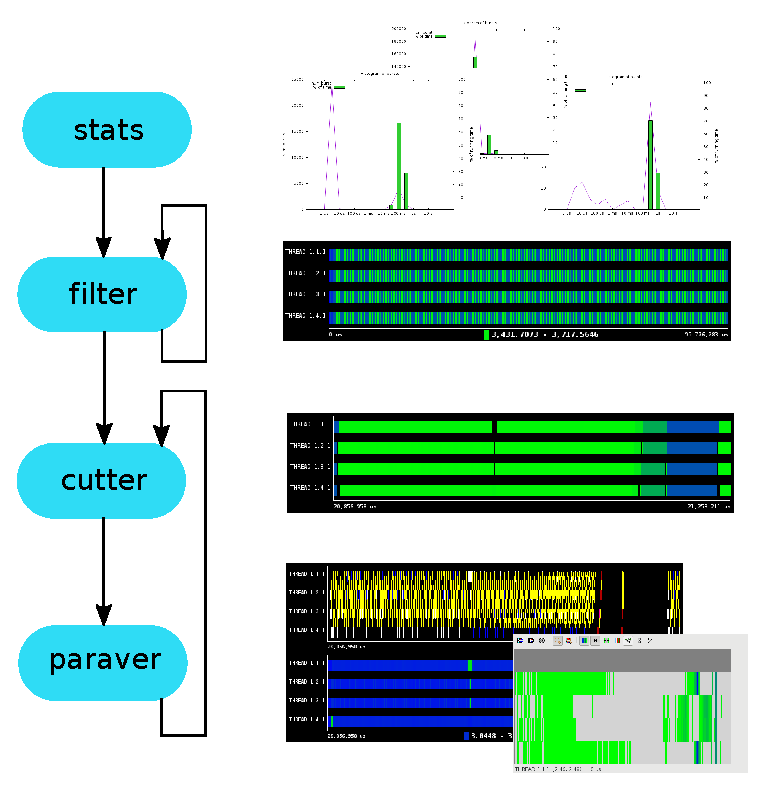
\includegraphics[width=250px]{current_analysis_flow.eps}
%\end{figure}

Talk about the BSC performance tools environment and introduce the analysis flow
with and without this proposed tool.

This is the mission of the parallel performance analysis. In an application-centric
approach, the performance analysis is a cyclic process consisting of observing 
the behaviour of the application so as to hypothesize the possible problems that 
affect its performance and finally translate these hypotheses to improvements in
the application re-starting the cycle to validate them. Obviously, the less number 
of iterations of this cycle the less time wasted and also the less money spent.


% NOTES
% .- Remember to demonstrate the interarrival time of different calls in the sam
%e loop body tend to be the same.


